\Aufgabe[e]{Nichtlineare Differentialgleichung erster Ordnung}
{
\begin{itemize}
\item[\textbf{1)}] Klassifizieren Sie die folgenden Differentialgleichungen erster 
Ordnung als 
\begin{enumerate}
\item Homogene Differentialgleichung: $y'=g(y/x)$ mit Substitution $u=y/x$.
\item Differentialgleichung mit bilinearen Argumenten: $y'=f(ax+by+c)$ mit Substitution $u=ax+by+c$.
\end{enumerate}
\begin{multicols}{2}
\begin{iii}
\item $\displaystyle y'(x^2+xy) = y^2-xy$,
\item $\displaystyle y' = \frac{x^2y}{x^3+y^3}$,
\item $\displaystyle y'=\frac{1}{x+y}$,
%\item $\displaystyle y'=\frac{2x-y}{x-2y}$,
\item $\displaystyle y'=-\sin^2(x+y+1)$,
\item $\displaystyle x^2y' = y^2+xy-x^2$,
\item $\displaystyle y'=\frac{y+\operatorname{e}^{-\frac{y}{x}}}{x}$
\end{iii}
\end{multicols}
\item[\textbf{2)}]  
Verwenden Sie eine angemessene Substitution und formulieren Sie die Gleichungen in Termen
von $u$ und $u'$ um ohne sie zu lösen.
\end{itemize}
}


\Loesung{
\begin{itemize}
\item[\textbf{1)}] 
\begin{iii}
\item $\displaystyle y'(x^2+xy) = y^2-xy$, homogen.
\item $\displaystyle y' = \frac{x^2y}{x^3+y^3}$, homogen.
\item $\displaystyle y'=\frac{1}{x+y}$, bilineare Argumente.
%\item $\displaystyle y'=\frac{2x-y}{x-2y}$, homogeneous.
\item $\displaystyle y'=-\sin^2(x+y+1)$, bilineare Argumente.
\item $\displaystyle x^2y' = y^2+xy-x^2$, homogen.
\item $\displaystyle y'=\frac{y+\operatorname{e}^{-\frac{y}{x}}}{x}$, homogen.
\end{iii}

\item[\textbf{2)}] 
\begin{iii}
\item Mit der Substitution $u=y/x$ erhalten wir
\begin{align*}
y'(x^2+xy) &= y^2-xy\\
y'&= \frac{y^2-xy}{x^2+xy}\\
y' &= \frac{y^2/x^2-y/x}{1+y/x}\\
y' &= \frac{u^2-u}{1+u}\\
y'&= u'x+u = \frac{u^2-u}{1+u}\\
u' &= \frac{1}{x}\left(\frac{u^2-u}{1+u} -u\right)\\
u' &= -\frac{1}{x}\frac{2u}{1+u}.
\end{align*}
Diese Gleichung kann durch Variablentrennung gelöst werden. Die Lösung wird in der Übung nicht verlangt, aber wir zeigen sie hier
um einen Fall einer nicht expliziten Lösung zu zeigen.
\begin{align*}
u' &= -\frac{1}{x}\frac{2u}{1+u}\\
\frac{1+u}{u}\d u & = -\frac{2}{x}\\
\int \frac{1+u}{u}\d u & = -\int \frac{2}{x}\\
\ln|u| + u &= \ln x^{-2} + C\\
\operatorname{e}^{\ln|u|} \cdot \operatorname{e}^u &= C \operatorname{e}^{\ln x^{-2}}\\
u\operatorname{e}^u &= \frac{C}{x^2}\\
\frac{y}{x}\operatorname{e}^\frac{y}{x} &= \frac{C}{x^2}\\
yx\operatorname{e}^\frac{y}{x} &= C.
\end{align*}
Die letzte Gleichung liefert die Lösung $y$ in impliziter Form. Die Lösung kann z.B. mit Matlab geplottet werden:
% 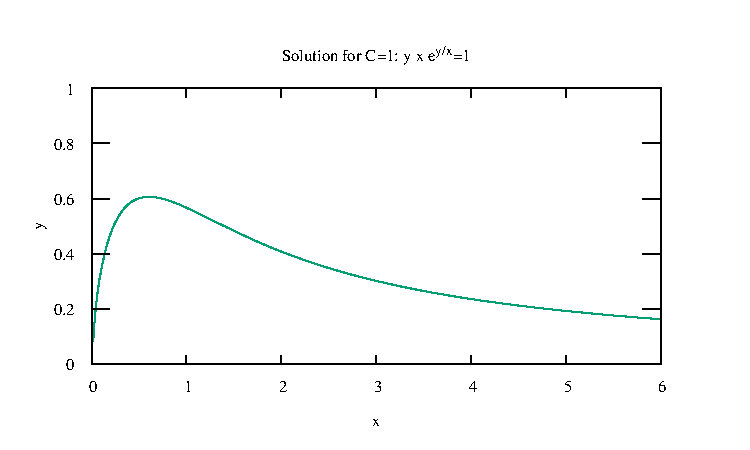
\includegraphics[width=0.5\textwidth] {../A/GewDgln/implicit_solution.pdf}
\item $\displaystyle y' = \frac{x^2y}{x^3+y^3}$.

Mit der Substitution $u=y/x$ erhalten wir:
\begin{align*}
y'&=\frac{x^2y}{x^3+y^3},\\
y'&=\frac{y/x}{1+y^3/x^3},\\
y'&=\frac{u}{1+u^3},\\
y'&=u'x+u = \frac{u}{1+u^3},\\
u'&= \frac{1}{x}\left( \frac{u}{1+u^3} - u\right),\\
u'&= -\frac{1}{x}\left( \frac{u^4}{1+u^3}\right).
\end{align*}
Die letzte Gleichung kann durch Variablentrennung gelöst werden und führt nach Rücksubstitution zu einer impliziten Gleichung für $y$.
\item $\displaystyle y'=\frac{1}{x+y}$.

Mit der Substitution $u=y+x$ erhalten wir:  
\begin{align*}
y'&=\frac{1}{u}\\
y'&=u'-1 =\frac{1}{u}\\
u' &= \frac{1+u}{u}.
\end{align*}
Die letzte Gleichung kann durch Variablentrennung gelöst werden und führt nach Rücksubstitution zu einer impliziten Gleichung für $y$.
\item $\displaystyle y'=-\sin^2(x+y+1)$.

Mit der Substitution $u=x+y+1$ erhalten wir:
\begin{align*}
y'&=-\sin^2(u)\\
y'&=u'-1 =-\sin^2(u)\\
u' &= \cos^2(u).
\end{align*}
Diese Gleichung kann mit Trennung der Variablen glöst werden (Die Lösung ist hier nicht gefordert):
\begin{align*}
u' &= \cos^2(u),\\
\frac{\d u}{\cos^2(u)} &= \d x,\\
\int \frac{\d u}{\cos^2(u)} &= \int \d x,\\
\tan(u) &= x+C,\\
u &= \arctan(x+C),\\
y+x+1 &= \arctan(x+C),\\
y &= \arctan(x+C)-x-1.
\end{align*}

\item $\displaystyle x^2y' = y^2+xy-x^2$.

Mit der Substitution $u=y/x$ erhalten wir 
\begin{align*}
y'&=\frac{y^2}{x^2}+\frac{y}{x} -1,\\
y'&=u'x+u = u^2+u-1,\\
u'&= \frac{u^2-1}{x}.
\end{align*}
Diese Gleichung kann z. B. durch Trennung der Variablen und partielle Bruchzerlegung gelöst werden.
\item $\displaystyle y'=\frac{y+\operatorname{e}^{-\frac{y}{x}}}{x}$.

Mit der Substitution $u=y/x$ erhalten wir

\begin{align*}
y'&=\frac{y}{x} + \frac{1}{x}\operatorname{e}^{-\frac{y}{x}},\\
y'&= u+\frac{1}{x}\operatorname{e}^{-u},\\
y'&= u'x+u = u+\frac{1}{x}\operatorname{e}^{-u},\\
u'&= \frac{1}{x^2}\operatorname{e}^{-u}.
\end{align*}
Das kann mit Trennung der Variablen gelöst werden.

\end{iii}

\end{itemize}
}



